\section{Vision}
The Nao vision system followed the process: \emph{Input image, classify image, form blobs, sort colour blobs, combine soft blobs, find ball, find goals, detect lines}. The 2009 vision module was an advancement over the 2008 module. This section details the main functions of the vision system and the reasons behind them. 

\subsection{Overview}

Webots was used to develop the base vision system in 2008. Inputting the RGB image and classifying it using a perfect look-up table (LUT) allowed blob formation and basic object recognition to be tested which then allowed for localisation development to begin. 

However this was not required in 2009, as the vision debugging application \emph{Eye of the NUbot} (EOTN) was already compatible with the robot directly. Advancements of EOTN carried over from last year were the HSI classification method. Transforming the YUV image to HSI values and selecting the classification region in HSI allowed for an intuitive classification method and better separation of hue ranges. 

The process of setting up a robot for a game includes setting the camera settings were selected using \emph{Telepathe}. Then obtaining image streams which were saved on the robot or could be transferred through the wireless interface to EOTN to be processed and examined. During examination of the images, the user could also generate a LUT using EOTN. Generating the LUT also enabled the user to check the classification and field object detection for errors. Before uploading the new LUT to the robot to use. This had to be completed for both top and bottom cameras.

Advancements that were included in the vision module this year were more ratio checks for the ball and goals, including a green horizon. This was to reduce the number of false objects recognised by the robots. We also included heuristics for the detection of new field objects, such as penalty spots, and the centre circle. These new field objects greatly enhanced the performance of the localisation module. Also, we increased the camera resolution from the minimal of 160x120 to an medium image of 320x240. This increased the accuracy of the object seen (example, a ball can be seen at the full length of the field), with a trade-off to robots processing speed. Also there was an additional camera added into the hardware system, in which we had to account for when processing the image.

%\emph{Input image, classify image, form blobs, sort colour blobs, combine soft blobs, find ball, find goals, line detection}


\subsection{Image Quality and Camera Settings}
%One good thing about the transition from the Aibo to the Nao was the improvement in camera quality. While the camera still had its share of problems, such as random swaps of U and V channels, random blackouts and random ghost camera settings, at least it made the separation of colours easier.
%The Nao has three different resolutions for which we could obtain images, 160x120, 320x240 and its native resolution 640x480. 
This year was the first year where we successfully started processing larger image resolutions. We increased the image resolution from 160x120 pixels to double the resolution, 320x240 pixels. This enabled clearer images and more accurate distances when we found recognisable objects. For example a ball could be detected by the goal keeper standing at its goal from the other end of the field. However, with higher resolution images the calculations to process an image became computationally heavy. This forced us to reduce our frame rate to 15 frames per second.

There was an additional camera installed around the nose of the Nao. This camera was particularly useful for lining up kicks. However, switching over from one to another would take time, which equates to the loose of a few frames. Logic was inserted in the search behaviour to reduce the number of camera transitions. 

\subsubsection{Camera settings}

The Nao camera has 6 main camera settings with a large range of values for each setting. This means that the camera settings are very sensitive to lighting changes and not only do colour tables need to be recalibrated for any change, but also the camera settings. At the RoboCup venue the camera settings and colour tables had to be recalibrated for both the main field and test fields. 

The robot is mobile with a movable head. This means that images are subject to blurring and lighting flare. Camera settings are chosen to minimise blurring and allow for best colour separation.

\subsection{Colour Classification}

Colour classification is the top tier in the software system. Any error in classification has a flow on effect to the entire system. Image pixels are mapped to a colour class by referencing a LUT. The environment of the Standard Platform League is colour coded so that objects are recognisable by colour. Rather than classify pixels based on object colour classes alone, additional `soft' colour classes are used to allow additional colour information to be classified and to reduce the risk of false positive classification.

\subsubsection{Soft Colour Classification}

Soft colour classification is used to classify regions of colour that belong to an object but is less saturated due to lighting conditions or overlaps with another colour class. This allows the decision about what object the soft colour belongs to, to be delayed until the entire image is processed.

Using soft colour allows for the classification of `noisy' shades of colour and allows valuable object size information to be kept. The risk of false positives is reduced by allowing true colour to be classed as the shades of colour that are highly saturated. Object decisions are based on the presence of true colour and then soft colour can be used for additional size information.

The shiny bright blue uniforms of the Nao have created a significant overlap of colour values with the blue goal. Similarly, the shiny red uniforms become less saturated with the reflection of light and the hue values shift closer to orange.

Soft colour is also applied to less saturated shades of colour. These shades are more likely to occur in background noise. Soft colour is used to classify additional bright and dark shades of red, orange, yellow and blue. 
 
Blobs are formed for each colour class, including soft colours. Once the image is processed soft colour decisions are made based on blob arrangement in Soft Colour Filtering. 

\subsection{Blob Formation}

Grouping of classified colours is used for the transfer of information from an image to object recognition. When forming blobs the colour, size and area information is required. Blobs are formed based on classified colour of the classified image. Undefined, white and field green and the soft colour shadow-black are not included in blob formation. This is due to the fact that size and shape information is not required for objects of these colours. It is also due to the nature of distribution of these colours. They are all abundantly spread throughout images and scattered; forming blobs on images would involve unnecessary processing. 

Blob formation checks every pixel of the image when forming blobs, this means we can form blobs as small as 1x1, however, we only use blobs greater than or equal to 3x3 pixels. 

\subsection{Sort Colour Blobs}

Soft colour blobs are filtered and kept if of sufficient size or overlapping with the corresponding true colour. During this stage, a simple check is also performed on the ball object. The ball must sit below the highest green transition (a simple green horizon) to be a valid ball.

\subsection{Combine Soft Blobs}

Overlapping soft colour blobs are merged. Colour blob clusters are then made to prepare information for object recognition. Cluster variables include: exists, correct pixels, colour 2 correct pixels, min x, max x, min y, max y, height, width, area. 
Yellow blobs, shadow yellow blobs and all yellow blobs are clustered for yellow goal recognition. Blue blobs, shadow blue blobs and all blue blobs are clustered for blue goal recognition and blue robot separation. Red blobs and shadow red blobs are clustered for red robot detection.

Clustering allows object recognition to have a region of interest. With the use of soft colour most goal images are made of multiple blobs.
\subsection{Ball Recognition}

Ball recognition was based on previous code. The main difference is that we don't have to deal with the up close ball situation. Instead we have to be able to see the ball at an elevated position and with additional glare shining off the ball. A confidence system is used to decide the ball. Confidence is weighted based on correct pixel to size ratio, size and circle fit.

\subsubsection{Ball Distance, Bearing and Elevation Calculations}
The raw values of bearing and elevation are calculated using the centre x and centre y of the blob in the image, while the raw
distance is calculated using the width of the blob in pixels. These resulting values are relative to the camera. They are then transformed using the forward kinematics of the robot to give a relative location in terms of the robots reference frame.

\subsubsection{Circle Fitting}

Least squares circle fitting has been implemented to improve the distances, bearings and elevations of balls that are not fully
visible in the image. There are two main parts to the circle fitting procedure. Firstly the selection of the points to be fit, followed by the fitting of a circle to these points. These points are gathered during one of various scan types depending on the positioning of the ball in the image. The points are found by searching from the outside of the blob inwards until it finds pixels of the same colour of the blob, or in the case of the orange blobs also one of the soft colours close to orange. The directions for which scans have been created are: \emph{Left to Right, Right to Left, Top to Bottom, Bottom to Top,Simultaneous Left to centre \& Right to centre and Simultaneous Top to Centre \& Bottom to Centre}. These can be seen in Figure~{\ref{fig:objectBall3}. The reason the different scanning directions are needed is so that in images in which the view of the ball is cut off by the edge of the image, points are not selected along the edge of the image in turn biasing the circle fit. For more information on the least squares fitting function used see [Seysener 2003; Seysener \emph{et al.} 2004].

\begin{figure}[!ht]
\begin{center}
    %\leavevmode
    \scalebox{0.3} {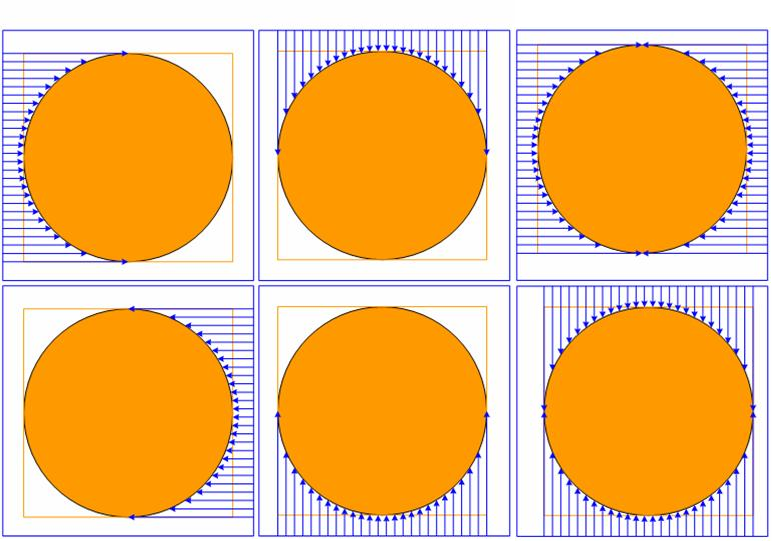
\includegraphics{stevenfigs/objectBall3.png} }
    \caption{Ball scanning directions,  (top left) left to right, (middle left) right to left, (bottom left) left and right to centre, (top right)  top to bottom, (middle right) bottom to top, (bottom right) top and bottom to centre.}
    \label{fig:objectBall3}
\end{center}
\end{figure}

Once a circle has been fit to these points, the validity of the fit circle is determined. If the diameter of the circle is significantly lower that the width of the blob then it is assumed that the circle fit is not correct.


\subsection{Goal Recognition}

With the use of soft colour classification and due to obstructions on the field, the goal is often not seen as a single blob, but rather a cluster of blobs. A scan method was used on clusters to detect the gap type and calculate the width of posts. 3 horizontal scan lines were used to detect gap type and post width by measuring the pattern of colour and soft colour compared to non object colours.

Gap types detected are: no gap (unknown post), left (right post), right (left post), middle (both posts, no crossbar), bottom (both posts and crossbar) or undefined. 

Three main variables were used to calculate goal confidence. Correct pixel to size ratio, cluster height to width ratio and goal gap detected. The amount of correct pixels required to pass as a goal object depends on the size and shape of the cluster and also what gap type it has. For instance an image of a single up close goal post will be detected as having no gap. Then it must pass a height to width ratio check and colour pixels to size ratio check to be recognised as a post. The ratio of correct pixels to size is different for each gap type.
 
\subsubsection{Goal Distance, Bearing and Elevation Calculations}

The raw distance of the goal is found by using the width of a post. With the new tall goals and the robot camera position looking down for a ball, the goal height is unreliable. If both goal posts are seen both widths are used to calculate the distance to each post. 

The raw bearing and elevation are found using the centre of the post. The method to find the centre of the post varies depending on the gap type. As with the ball these raw distances are translated back so they are relative to the hips of the robot. The elevation is not very reliable as the top of the post is often not seen.

%\subsection{Robot Recognition}
%
%Red robots are detected by clusters of red blobs. Blue robots are detected using the clusters of shadow blue blobs if blue goal tests have failed.





\subsection{Line and Corner Point Detection}

This year the algorithm used in previous years to detect field lines and corners  [Quinlan \emph{et al.}, 2006] was ported from the Aibo to the new Nao system. This required rewriting the function that transforms the found corner points in the camera plane to the field plane to suit the new robot kinematics and camera perspective. Otherwise, the algorithm is the same as the previous years for detection. Further development this year involved uniquely identifying these found corner points for use in Localization.

\subsubsection{Line Detection}
The detection of field lines is approached in a completely different manner to that of other Objects. When searching for objects, sections of a specific colour are joined together to form a blob. While this works well for most objects, white causes problems due to its abundance in the image and hence is normally ignored. Also the thin nature of lines, and the robot's low Point Of View, makes missing pixels very common within the classified image. Finally the storing of blobs, as a square which bounds the entire object, does not store enough important information about the line.

To overcome these issues the detection of lines is based around the two unique features that field lines have; their long thin length and their green-white-green transitions. Using these two details the image can be sparsely searched, since the search line does not need to find every point of the line, just enough to re-create the line. Also the transition information allows many white pixels to be thrown out early in the detection process, thereby reducing the overall load on the processor. This reliance on points and not the entire line also allows the lines to be partially hidden behind another object without effecting their detection. 

With these factors in mind, the image can now be efficiently searched in the following steps;

\begin{itemize}

\item 	The image is searched using a horizontal and vertical search grid. The search is restricted to the area in the image below the horizon line and picks out points of sharp contrast which have green-white then white-green transitions. These points are recorded in an array for later use.

\item The found points are then checked against each other to form possible lines. Once candidates are found, more points are checked and added until a line is formed. All checks on the lines at this stage is done based on gradient to allow the fastest line formation.

\item The lines are cleaned up to make sure all points actually fit on the line. Lines which have too large a number of points not contained within the final line are removed.

\item Lines are checked against each other to confirm that they are not just segments of larger lines. The allows lines to be formed that have a break in the middle, such as when a robot is on top of the line.

\item Corner points are found by extending lines and finding their intersection locations. The intersections are checked to confirm virtual points are not found. 

\item An attempt is made to uniquely identify corner points from other objects within the image. While this is not always needed, if a unique identification is made the use of the corner point within localisation becomes much more efficient.

\end{itemize}

\subsubsection{Corner Point Detection}
The locating of these corner points alone in each frame is not enough to localize with as there are numerous type-L and type-T corners on each side and a complete mirror image of the field lines on each half end of the field. Unique identification of each corner point is required in our system. A rule based approach was used to perform this identification that filters out the possible corner identity based on what properties of the corner can be extracted from the image and in most cases also some vague knowledge of robot location and orientation. 

The goal was not to provide data that Localization can rely upon solely but to fine tune the accuracy once approximate localization has been established. However this use of knowledge of location and orientation creates a loop between the Line Detection and Localization system components. This allows for the possibility of each component validating each other's incorrect data to exist. This being the case, the main focus was to write identification rules that are strict enough to eliminate the possibility of false positives. Also, the corner point identification rule written would block (that is, return an unknown corner or T point) unless the Localization confidence first came within 2 standard deviations of the probable orientation.
      
The identification relies upon the orientation of the seen corners, the combination of these corners and other lines in the image and the number of corners and lines seen. The Line Detection algorithm classifies each corner as either a type L or T and then attributes it with one of four possible orientations, pointing up/down or pointing left/right. By disassembling the field lines in the image they could be examined for what types of corners and orientations make up what is seen. Following that, this information is then decoded to match what should be seen from the present known location. Avoiding false positives here partially takes care of itself as if the robot location or orientation data is wrong, the corresponding corner orientation classification will not match the rule.

For example, in Figure \ref{fig:corner}a taken from the simulator, the detection algorithm reports seeing 3 corners: 2 type L's of orientation 2 and 4, 1 type T of orientation 1 and 4 lines. This set of data is almost unique when compared to the other countless possible positions and perspectives from which to view the field lines and can therefore be decoded with brute force. 
 
The only other occurrence is a duplicate on the opposite end of the field as both halves are identical. This the leaves the question, "which end of the field is the robot in?". Knowledge of the robots orientation could also solve this problem of determining which end of the field this scene is taken from. To be robust, the rules written require Localization to be certain of both field XY position and orientations to 2 standard deviations. This value could be increased in this case but for others closer to the mid field line, the probability of error increases as the two mirror images from each end come closer together. The necessity for this prior knowledge is best show pictorially.
    
In the first frame we have no other information to work with other than the lines themselves. In the second frame, the Goal Detection provides Localisation with enough information to determine which end of the field the robot is in and it is now possible to uniquely identify the corner points.
      
Another example of an identification rule would the identification of a mid field T corner. Conditional tests for seeing only: 2 field lines, corner count = 1, corner type = T, corner orientation = 3, robot X location is greater than zero, orientation is 135 degrees plus or minus 80 degrees and no goal post is seen, accurately reports the correct corner and filters out all others.
      
Unique identification rules were written for each corner for a selection of possible perspectives and rigorously tested in the Webots simulator. Possible sources of error discovered in testing were the extension of the penalty box line to join the side field line to create a phantom type T corner, the clipping of a type T corner into a type L by the edge of the camera frame and the center circle appears as a collection of many corners (for example an octagon). Each of these sources of error were reliably filtered out by the corner combination decoding.
      
The simulation testing also showed great improvement in Localisation over simply relying upon goal detection alone. Once a goal had been seen and Localisation determined to some approximate area, the line detection would report a unique corner point and fix a very accurate position and orientation and maintain it while looking all around the field. 

The identified point on the field is then sent to Localization after performing the following transformation.

$V_{cam}=[focLength, (IMG_{width}/2)- X_{img},(IMG_{height}/2)-{Y_{img}}]$

Transformation through neck

\textbf{$V_{1}$}=\textbf{$V_{cam}$}*\textbf{$M_{camTilt}$}

\textbf{$V_{2}$}=\textbf{$V_{1}$}*\textbf{$M_{camPan}$}

Transform body tilt

\textbf{$V_{3}$}=\textbf{$V_{2}$}*\textbf{$M_{bodyTilt}$}

$\alpha=-Chest Height/V_{3}[2]$

$distance=\alpha*\sqrt{V_{3}[0]^2+V_{3}[1]^2}$

$bearing=arctan2(V_{3}[0],V_{3}[1])$

This inter system approach to the corner identification is shown in Figure \ref{fig:corner} b and c. Green components demonstrate an improvement to this approach where one of the Localisation reset triggers becomes an external one based on an added component that monitors for robot relocation by hand by way of accelerometer readings (Teleport Detection if image is BW). In the Robocup competition robots do get picked up and moved, possibly to the other side of the field and turned around by 180 degrees when being penalized. The loop created between the Line Detection and Localisation could slow down the reset as it would take some time for the bad data to be dumped after locating a goal post and dealing with conflicting information. A specialised system component could ensure this does not happen.
\begin{figure}[htpb]
\begin{center}
    %\leavevmode
    \scalebox{0.3} {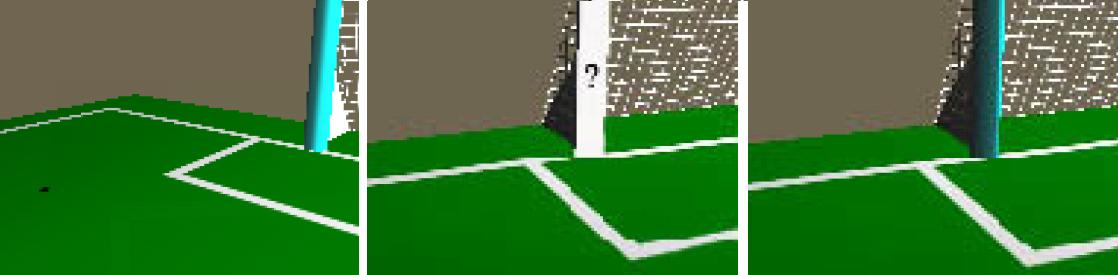
\includegraphics{alexfigs/corner.png} }
    \caption{Images of corners for examples.}
    \label{fig:corner}
\end{center}
\end{figure}

%\subsubsection{Code Implementation}
%Up until this year, Line Detection was a collection of functions within the Vision class itself. To
%reduce coupling, the Line Detection function and supporting functions were removed from the vision
%class and placed into a newly created Line Detection class. This Line Detection class is responsible for
%both line detection and the corner identification. These routines are still part of the vision system and
%the files can be found in the vision directory. No other NUManoids system component is dependent
%upon this Line Detection class to in order run and therefore it may be removed from the project build by
%editing the MakeFile in the root of the code body.
%Once a Line Detection object has been instantiated, the Line Detection function �formlines()� is
%called at the end ProcessFrame() within the class Nao. It requires no data to be passed into it and it
%outputs its results by directly modifying the elements found in the �fieldObjects� structure. The list of all
%possible corner points that can be evaluated can be found in the FieldObject.h file.
%\begin{figure}[!ht]
%\begin{center}
%    %\leavevmode
%    \scalebox{0.3} {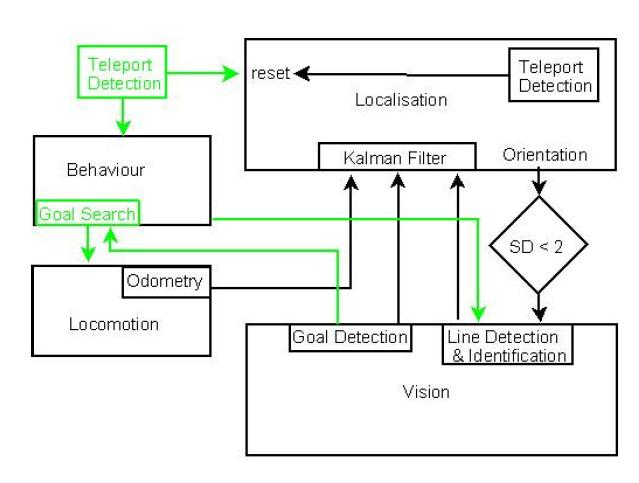
\includegraphics{alexfigs/flow.png} }
%    \caption{Software flow diagram.}
%    \label{fig:flow}
%\end{center}
%\end{figure}


\subsubsection{Penalty Spot Detection}
Penalty spots exists in two positions on the field. By detecting any penalty spot, localisation module has a higher chance of knowing where the robot is currently situated on the field. Detecting the penalty spot consists of a search heuristic:
\begin{itemize}
\item Find lines that are less then a quarter length of the screen: If a standing robot should see a penalty spot, it should be relatively small on the screen.
\item Using the points on the selected line, we scan around each of these line points for surrounding white colours:
This scan consists of a 3x3 grid search around the selected point.
\item If there does not exist to be any white colours, its most likely to be a penalty spot, Otherwise it is not a penalty spot.
\end{itemize}
This is a simple and efficient heuristic, because the priori conditions make the search space is very small.

\subsubsection{Centre Circle Detection}
Centre circle is an a very important field object on the SPL field. This object is so big that almost from any section of the field (provided that is facing inwards). It enhances and assists the localisation module greatly, due to its visibility and unambiguous properties of the object. To detect a centre circle, there exists two steps. First Step, is to remove points that do not belong on the centre circle. Second step, consists of an least squares approach to fit the points of the centre circle to an ellipse equation.
Once this is complete, we are able to obtain the ellipse, and the robots current distance to it.

The first step is removing points that do not belong on the centre circle, this is achieved by an heuristic. Here we assume that after all points have been fitted to a line, corners (intersections) of lines have been calculated and all penalty spots have already been detected. Here we assume a centre circle consists of many small straight lines, with many straight lines these should intersect on screen a large number of times. Assuming a number of corner tolerance of six, if the number of corners are greater then six, centre circle detection will be triggered. 
\begin{itemize}
\item Find the longest line (most likely to be the centre line) and remove it from the search list.
\item Find the Penalty Spot lines and remove it from the search list.
\item Assuming that the lines are small, we select all the small lines. For our system, a small line is a line that is less the image width.
\item We then select the line points that exist within these lines and store them in a vector ready to be processed by the next stage.
\end{itemize}

The next stage consists of fitting the obtained points to an ellipse equation. By fitting the points to an equation we are able to generalise and efficiently store the data of the ellipse for later use. The ellipse fitting algorithm is an implementation of 